\section{Multitask Training for Recommender Systems}

In this assignment, we will implement a multi-task movie recommender system based on the classic Matrix Factorization \cite{Yehuda2009matrix} and Neural Collaborative Filtering ~\cite{he2017neural} algorithms. In particular, we will build a model based on the \href{https://www2.seas.gwu.edu/~simhaweb/champalg/cf/papers/KorenBellKor2009.pdf}{BellKor solution} to the Netflix Grand Prize challenge and extend it to predict both likely user-movie interactions and potential scores. In this assignment you will implement a multi-task neural network architecture and explore the effect of parameter sharing and loss weighting on model performance.

\vspace{0.2cm}
\noindent The main goal of these exercises is to familiarize yourself with multi-task architectures, the training pipeline, and coding in PyTorch. These skills will be important in the course. \textbf{Note: This assignment is a warmup, and is shorter than future homeworks will be.}

\vspace{0.2cm}

\noindent\textbf{Code Overview:} The code consists of several files; however, you will only need to interact with two:

\begin{itemize}
    \item \texttt{main.py}: To run experiments, execute this file by passing the corresponding parameters. 
    \item \texttt{submission.py}: This file contains our multi-task prediction model \textbf{MultiTaskNet}, which you will need to finish implementing in PyTorch.
\end{itemize}

\textbf{Dataset} In this assignment, we will use movie reviews from the \href{https://grouplens.org/datasets/movielens/100k}{MovieLense dataset}. The dataset consists of 100K reviews of 1700 movies generated by 1000 users. Although each user interaction contains several levels of meta-data, we'll only consider tuples of the type \textbf{(userID, itemID, rating)}, which contain an anonymized user ID, movie ID and the score assigned by the user to the movie from 1 to 5. We randomly split the dataset into a \textbf{train} dataset, which contains 95\% of all ratings, and a \textbf{test} dataset, which contains the remaining 5\%.

\textbf{Problem Definition}
Given the dataset defined above, we would like to train a model $f(\text{userID}, \text{itemID})$ that predicts: 1) the probability $p$ that the user would watch the movie and 2) the score $r$ they would assign to it from 1 to 5. For some intuition on this setting, consider a user who only watches comedy and action movies. It would not make sense to recommend them a horror movie since they don't watch those. At the same time, we would want to recommend comedy or action movies that the user is likely to score highly. 

\textbf{Evaluation}
Once we have our trained model, we evaluate it on the test set.

\vspace{0.2cm}
\textbf{Score Prediction} We will evaluate the mean-squared error of movie score prediction on the held-out user ratings, i.e.
    $
        \frac{1}{N}\sum_{i=1}^N \|\hat{r}_i-r_i\|^2,
    $
    where $\hat{r}_i$ is the predicted score for user-movie pair $(\text{userID}_i,\text{itemID}_i)$. The summation is over all pairs in the test set. Better models achieve lower mean-squared errors.
    
\vspace{0.2cm}
\noindent \textbf{Likelihood Prediction}  
% Our dataset contains ratings for movies the users have seen. 
To evaluate the quality of the likelihood model, we use the \href{https://en.wikipedia.org/wiki/Mean_reciprocal_rank} {mean reciprocal rank metric}, which provides a higher score for highly ranking the movies the user has seen. The metric is computed as follows: 
\begin{enumerate}
    \item For each user, rank all movies based on the probability that the user would watch them
    \item Remove movies we know the user has watched (those in the training set)
    \item Compute the average reciprocal ranking of movies the user has watched from the held-out set
\end{enumerate} 

\vspace{0.2cm}
\noindent\textbf{Matrix Factorization}
Consider an interaction matrix $M$, where $M_{ij} = 1$ if $\text{userID}_i$ has rated movie with $\text{itemID}_j$ and $0$ otherwise. We will represent each user with a latent vector $\mathbf{u}_i\in\mathbb{R}^d$ and each item with a latent vector $\mathbf{q}_i\in\mathbb{R}^d$. We model the interaction probability $p_{ij}=\log P(M_{ij}=1)$ in the following way:
\begin{equation}
    p_{ij} = \mathbf{u}_i^T\mathbf{q}_j + a_i + b_j
    \label{eq:prob}
\end{equation}
where $a_i$ is a user-specific bias term and $b_j$ is a movie-specific bias term. At each training step we sample a batch of triples $(\text{userID}_i, \text{itemID}_j^+, \text{itemID}_{j'}^-)$ with size $B$, such that $M_{i, j} = 1$, while $\text{itemID}_{j'}^-$ is randomly sampled (indicating no user preference). Note the $+$ and $-$ refers to the positive and negative sample. The positive example means the correctly paired $\text{itemID}$ for the user, and the negative sample is the randomly sampled one. Let
\begin{equation} 
    \begin{split}
        p^+_{ij} =  \mathbf{u}_i^T\mathbf{q}_j + a_i + b_j \\
        p^-_{ij'} =  \mathbf{u}_i^T\mathbf{q}_{j'} + a_i + b_{j'}
    \end{split}
\label{eq:p}
\end{equation}
and optimize the  Bayesian Personalised Ranking (BPR) \cite{Rendle2009BPR} pairwise loss function:
\begin{equation}
    \mathcal{L}_F(\mathbf{p}^+, \mathbf{p}^-)=\frac{1}{B}\sum_{i=1}^B 1-\sigma(p_{ij}^+-p_{ij'}^-)
    \label{eq:l1}
\end{equation}

 where $\sigma$ is the sigmoid function.

\vspace{0.2cm}
\noindent\textbf{Regression Model}: For training the regression model, we consider only batches of tuples $(\text{userID}_i, \text{itemID}_j^+, r_{ij})$, such that $M_{i, j} = 1$ and $r_{ij}$ is the numerical rating $\text{userID}_i$ assigned to $\text{itemID}_j^+$. Using the same latent vector representations as before, we will concatenate $[\mathbf{u}_i, \mathbf{q}_j, \mathbf{u}_i * \mathbf{q}_j]$ (where $*$ denotes element-wise multiplication) together and pass it through a neural network with a single hidden layer:
\begin{equation}
    \hat{r}_{ij}=f_{\theta}([\mathbf{u}_i, \mathbf{q}_j, \mathbf{u}_i * \mathbf{q}_j])
    \label{eq:reg}
\end{equation}
We train the model using the mean-squared error loss:
\begin{equation}
    \mathcal{L}_R(\mathbf{\hat{r}}, \mathbf{r})= \frac{1}{B}\sum_{i=1}^B \|\hat{r}_{ij}-r_{ij}\|^2
    \label{eq:r}
\end{equation}

\begin{enumerate}
	\item {\bf Implement MultiTaskNet Model}

The first part of the assignment is to implement the above model in \texttt{submission.py}. First you need to define each component when the model is initialized. 

\begin{enumerate}
    \item \points{1a} Consider the matrix $\mathbf{U} = [\mathbf{u}_1\mid,\ldots,\mid \mathbf{u}_{N_{\text{users}}}]\in\mathbb{R}^{N_{\text{users}}\times d}$, $\mathbf{Q} = [\mathbf{q}_1\mid,\ldots,\mid\mathbf{q}_{N_{\text{items}}}]\in\mathbb{R}^{N_{\text{items}}\times d}$, $\mathbf{A} = [a_1, \ldots, a_{N_{\text{users}}}]\in \mathbb{R}^{N_{\text{users}}\times 1}$, $\mathbf{B} = [b_1, \ldots, b_{N_{\text{items}}}]\in \mathbb{R}^{N_{\text{items}}\times 1}$. Implement $\mathbf{U}$ and $\mathbf{Q}$ as \texttt{ScaledEmbedding} layers  with parameter $d=\texttt{embedding\_dim}$ and $\mathbf{A}$ and $\mathbf{B}$ as \texttt{ZeroEmbedding} layers with parameter $d=1$ (defined in \texttt{models.py}). These are instances of \href{https://pytorch.org/docs/stable/generated/torch.nn.Embedding.html}{PyTorch Embedding} layers with a different weight initialization, which facilitates better convergence.
    When \texttt{embedding\_sharing=False} we will set separate latent vector representations used in the distinct factorization and regression tasks $\mathbf{U_{reg}}, \mathbf{U_{fact}}, \mathbf{Q_{reg}}, \mathbf{U_{fact}}$ of similar type and dimensions of $\mathbf{U}, \mathbf{Q}$. 
    
    Please complete the following functions in \texttt{submission.py}:
    \begin{enumerate}
        \item \texttt{init\_shared\_user\_and\_item\_embeddings}
        \item \texttt{init\_separate\_user\_and\_item\_embeddings}
        \item \texttt{init\_user\_and\_item\_bias}
    \end{enumerate}

    \item \points{1b} Next implement $f_{\theta}([\mathbf{u}_i, \mathbf{q}_j, \mathbf{u}_i * \mathbf{q}_j])$ as an MLP network. The class \texttt{MultiTaskNet} has \texttt{layer\_sizes} argument, which is a list of the input shapes of each dense layer. Notice that by default $\texttt{embedding\_dim}$=32, while the input size of the first layer is 96, since we concatenate $[\mathbf{u}_i, \mathbf{q}_j, \mathbf{u}_i * \mathbf{q}_j]$ before processing it through the network. Each layer (except the final layer) should be followed by a ReLU activation. The final layer should output the final user-item predicted score in and have an output size of 1. Please complete the \texttt{init\_mlp\_layers} function in \texttt{submission.py}.
\end{enumerate}
    \item \points{2} {\bf Implement Forward}

In the second part of the problem you need to implement 
the \texttt{forward\_with\_embedding\_sharing} and 

\texttt{forward\_without\_embedding\_sharing} methods of the 
\texttt{MultitaskNet} module. 


Both forward methods above receive a batch of $(\text{userID}_i, \text{itemID}_j)$ 
of user-item pairs. The model should output a probability $p_{ij}$ of 
shape $(batch\_size,)$ that user $i$ would watch movie $j$, 
given by Eq. \ref{eq:prob} and a predicted score $\hat{r}_{ij}$ 
of shape $(batch\_size,)$ the user $i$ would assign to movie $j$, 
given by Eq. \ref{eq:reg}. 

\textbf{Be careful with output tensor shapes!}

\clearpage

    \item {\bf Experiments}

To execute experiments, we will run the \texttt{run\_all.sh} script, which will automatically log training MSE loss, BPR loss and test set MSE loss and MRR scores to TensorBoard. Once you're done with your implementation run the following 4 experiments:

Here the \texttt{--factorization\_weight} and \texttt{--regression\_weight} arguments correspond to $\lambda_F$ and  $\lambda_R$ respectively.

As you run the commands below, ensure to run \texttt{tensorboard --logdir=run} in another terminal to view training progress across experiments on your \href{http://localhost:6006/}{localhost:6006}. Note that you can also run \texttt{--device} to specify running on gpu or cpu and add \texttt{--debug=True} to view console output training progress.

\begin{enumerate}[I]
    \item Evaluate a model with shared representations and task weights $\lambda_F=0.99, \lambda_R=0.01$. You can run this experiment by running:
    
    \begin{verbatim}
        python main.py --factorization_weight 0.99 --regression_weight 0.01 
        --logdir run/shared=True_LF=0.99_LR=0.01
    \end{verbatim}    
    
    \item Evaluate a model with shared representations and task weights $\lambda_F=0.5, \lambda_R=0.5$. You can run this experiment by running:    

    \begin{verbatim}
        python main.py --factorization_weight 0.5 --regression_weight 0.5
        --logdir run/shared=True_LF=0.5_LR=0.5
    \end{verbatim}
        
    \item Evaluate a model with \textbf{separate} representations and task weights $\lambda_F=0.5, \lambda_R=0.5$. You can run this experiment by running:    

    \begin{verbatim}
        python main.py --no_shared_embeddings --factorization_weight 0.5
        --regression_weight 0.5 --logdir run/shared=False_LF=0.5_LR=0.5
    \end{verbatim}
        
    \item Evaluate a model with \textbf{separate} representations and task weights $\lambda_F=0.99, \lambda_R=0.01$. You can run this experiment by running:    

    \begin{verbatim}
        python main.py --no_shared_embeddings --factorization_weight 0.99
        --regression_weight 0.01 --logdir run/shared=False_LF=0.99_LR=0.01
    \end{verbatim} 
        
\end{enumerate}

After running all experiments above, you should generate graphs that look like

\begin{figure}[ht]
    \subcaptionbox*{MSE}[.45\linewidth]{%
        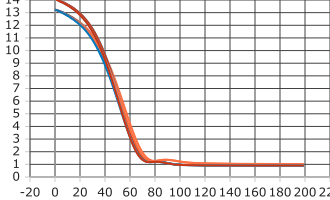
\includegraphics[width=\linewidth]{./figures/eval_MSE}%
    }%
    \hfill
    \subcaptionbox*{Mean Reciprocal Rank}[.45\linewidth]{%
        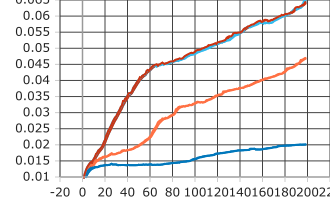
\includegraphics[width=\linewidth]{./figures/eval_Mean_Reciprocal_Rank}%
    }
    \caption{Evaluation Results}
\end{figure}

\begin{figure}[ht]
    \subcaptionbox*{Factorization Loss}[.33\linewidth]{%
        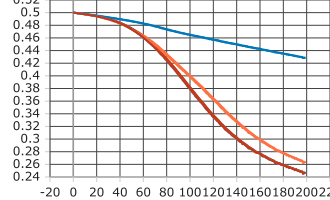
\includegraphics[width=\linewidth]{./figures/training_Factorization_Loss}%
    }
    \subcaptionbox*{Joint Loss}[.33\linewidth]{%
        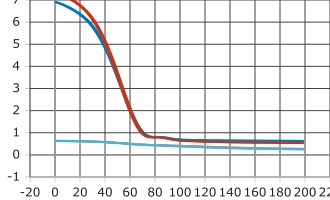
\includegraphics[width=\linewidth]{./figures/training_Joint_Loss}%
    }
    \subcaptionbox*{MSE}[.33\linewidth]{%
    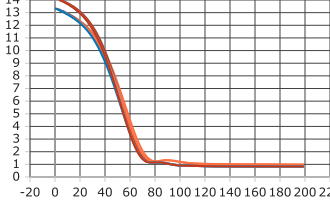
\includegraphics[width=\linewidth]{./figures/training_MSE}%
}%
    \caption{Training Results}
    \medskip
    \small
    \begin{center}
        \textcolor{orange}{Orange:} \texttt{shared=True\_LF=0.99\_LR=0.01}\\
        \textcolor{blue}{Dark Blue:} \texttt{shared=True\_LF=0.5\_LR=0.5}\\
        \textcolor{red}{Red:} \texttt{shared=False\_LF=0.5\_LR=0.5}\\
        \textcolor{cyan}{Light Blue:} \texttt{shared=False\_LF=0.99\_LR=0.01}
    \end{center}
\end{figure}


\begin{enumerate}
    \item \points{3a} Consider the case with $\lambda_F=0.99$ and $\lambda_R=0.01$. Based on the train/test loss curves, does parameter sharing outperform having separate models? 
    
    \item \points{3b} Now consider the case with $\lambda_F=0.5$ and $\lambda_R=0.5$.  Based on the train/test loss curves, does parameter sharing outperform having separate models? 
    
    \item \points{3c} In the \textbf{shared model setting} compare results for $\lambda_F=0.99$ and $\lambda_R=0.01$ and $\lambda_F=0.5$ and $\lambda_R=0.5$, can you explain the difference in performance?
\end{enumerate}
\end{enumerate}

\textbf{Coding Deliverables}

For this assignment, please submit the following files to gradescope to recieve points for coding questions:
\begin{itemize}
    \item |submission.pdf|
    \item |src/submission.py|
    \item |src/experiments_1.npy|
    \item |src/experiments_2.npy|
    \item |src/experiments_3.npy|
    \item |src/experiments_4.npy|
\end{itemize}
